\chapter{FG Nup aggregation under crowded conditions}\label{ch05}

Disordered proteins are often prone to aggregation, often causing disease, and the aggregation behavior of FG Nups is important to understand.  It is not clear what the aggregation state of Nups is within the pore or how their aggregation might play into nuclear transport \cite{things}.  \textit{In vitro}, many Nups spontaneously aggregate into amyoids over the course of a few hours, but there is evidence that this aggregation does not happen in the cellular environment \cite{frey07, Loren's paper}.  We investigated aggregation behavoir of an aggregation-prone Nup fragment in a number of different crowders.  Inert crowders such as PEG and PVP help mimic the extremely crowded cellular environment, but they may interact different with the protein than nonspecifically-binding crowders such as cell lysate or BSA.  We wanted to understand how different crowders affected the aggregation properties of Nups.

We used a 124-amino-acid fragment of the Nup Nsp1.  The FG-repeat segment of Nsp1 contains an aggregation-resistant portion (used as the basis for the FSFG peptide) as well as one that aggregates in buffer over the course of a few hours.  This aggregation-prone portion is the basis of the FG124 peptide used in the following aggregation experiments.

We used aggregation timecourses with thioflavin T as a readout, as well as fluorimetry, NMR, and x-ray scattering.  Our conclusion is something about the phenylalanines and how they behave differently in when crowded with PEG than with PVP (which also has an aromatic ring).

need an intro kind of figure with amyloid structure, cartoon of aggregation

\section{Fluorescence time courses}

In order to probe the aggregation dynamics of FG124, we incubated samples in the presence of crowders and thioflavin T (ThT), a dye which is sensitive to the presence of amyloids.  Over the course of several hours, FG124 aggregated and the fluorescence intensity from ThT increased.  By recording the intensity at 10-minute intervals, we were able to plot sigmoidal aggregation curves for the samples, as shown in Fig.~\ref{fig:sigmoid-fit}.  These curves show a lag phase while the aggregates are nucleating, followed by a growth phase of rapid aggregation, ending in a plateau phase.  We recorded timecourses for multiple crowders and analyzed the resulting aggregation parameters.

Thioflavin T is a dye that grows much brighter when bound to amyloids.  Upon binding, its absorption maximum shifts from from 385 nm to 450 nm and it emission maximum from 445 nm to 482 nm \cite{picken12}.  Although ThT is a more reliable indicator of amyloids than other fluorescence methods, notably Congo red stain, it suffers from reproducibility problems.  There is no consensus on the mechanism of ThT binding to amyloids.  Some proposed mechanisms rely on the presence of ThT micelles, which form above a critical concentration of about 4 $\mu$M, while others advocate for avoiding micelles \cite{khurana05, groenning09}.  There is some evidence that amyloid fibrils can adsorb to the plastic surface of a multiwell plate, decreasing ThT fluorescence intensity as the fibrils mature \cite{murray13}.  Often in our timecourse experiments, the ThT fluorescence did reach a maximum and then decrease.  The fluorescence intensity also depends on the sample viscosity, an effect which we noticed in our timecourses \cite{}.  Despite these challenges, thioflavin T is the most consistent dye for detecting the process of amyloid formation.

%basename = '/Users/lauramaguire/Google Drive/Hough Lab/Nuclear Pore Team/Data/FG124 aggregation timecourses/';
% Date in 'yymmdd' format
%date = '170126';
%13% PEG rep 3
\begin{SCfigure}
\caption{Sample sigmoid fit to FG124 sample with 13\% w/v PEG.  Burst phase and stationary phase are shown; lag phase took place before data collection began.  Fit is to Eqn.~\ref{eq:sig-fit}.\\}
\centering
\includegraphics[width=0.5\textwidth]{figs/ch05/sample-sigmoid}
\label{fig:sigmoid-fit}
\end{SCfigure}

\subsection{Methods}

\subsubsection{Buffers} Potassium transport buffer (PTB) (150 mM KCl, 20 mM HEPES, 2 mM $\tx{MgCl}_2$) was used for all timecourse and NMR samples.

\subsubsection{FG124 preparation} His-tagged FG124 was expressed in \emph{E. coli} in the plasmid pRSF.  Cultures were grown in LB and  induced at 37 degrees C for 2-4 hr with 1 mM IPTG at OD 0.6-0.8.  Periplasmic matrix was removed prior to lysis.  Cells were then lysed via sonication and FG124 purified using TALON cobalt resin.  All purification buffers were PTB with 7M GuHCl and PIC.  The elution buffer also contained 250 mM imidazole.

\subsubsection{Timecourse preparation} Stocks of PEG and PVP in PTB were prepared at 20 or 40\% w/v; serine stocks were prepared at 30\% w/v.  PEG and serine were at pH 7; PVP was pH 7 or pH 5.  Lyophilized lysate was prepared by homogenizing BL21 DE3 Gold cells and spinning them down.  The supernatant was lyophilized in a decomposing ammonium bicarbonate buffer and resuspended in PTB to the desired concentration when needed.  A 10 mM stock solution of ThT in PTB was prepared and filtered no more than a week before the timecourse, stored at room temperature and protected from light.  Immediately prior to starting the timecourse, FG124 was desalted into PTB to remove the imidazole and GuHCl.  Samples were promptly prepared containing the appropriate percentage of crowder, a final concentration of 1-2 mg/mL FG124, and 200 uM thioflavin T.  All samples in the same timecourse had the same concentration of FG124, including the buffer sample, which contained no crowding agent.  Blanks were prepared with crowding agent and thioflavin T, but no FG124.  Samples were pipetted into black, flat-bottomed, clear-bottomed 96-well plates with 150 uL per replicate.  Each sample yielded four to six replicates.  Only one blank replicate was used per condition.  One negative control and corresponding blank were prepared per timecourse containing 7M GuHCl and no crowding agent but using the same protein sample as all other conditions.  Each well contained a 3mm-diameter glass or teflon bead.  The plate was sealed with a PCR seal and taken to a Safire II plate reader.  The fluoresence was measured from the bottom at 10-minute intervals with an excitation wavelength of 450 nm, emission wavelength of 482 nm, and 5 nm bandwidths.  The plate shoook orbitally at high speed between measurements and was held at a temperature of 30 degrees C.  The time between desalting and beginning the plate reader measurements was typically about an hour; the time of desalting was taken as $t=0$ for the purposes of calculating lag time. In parallel with the sample preparation, the concentration of the desalted FG124 was measured with a BCA assay.

\subsubsection{Timecourse analysis}

After carrying out the aggregation timecourse, the data were normalized and fit to a sigmoid function in order to extract aggregation lifetimes and lag times.

The data were first normalized to the blanks, which contained crowding agents but no protein.  In nearly all cases, the blank intensity remained steady over time, as expected.  In those cases, the mean blank intensity was subtracted from the corresponding data.  In cases where the blank intensity changed over time, it was subtracted pointwise from the data.

Then the normalized curves were fit to a sigmoid given by
\begin{equation}
I(t) = C + \frac{A}{1+\exp \left(-k(t-T_{1/2})\right)}
\label{eq:sig-fit}
\end{equation}
where $I(t)$ is the normalized fluoresence intensity as a function of time.  The aggregation dynamics are described by the rate $k$ and the half-time $T_{1/2}$, which reflects the time needed for the intensity to reach half of its asympotic value.  More descriptive than the half-time is the lag time $T_\ell$, calculated as
\begin{equation}
T_l = T_{1/2} - \frac{2}{k}
\end{equation}
and representing the duration of the lag phase \cite{arosio15}.  The lag time here is defined as the intersection of the tangent line of maximum slope of the growth phase with the flat background signal of the lag phase.  

The offset $C$ and final amplitude $A$ are less meaningful in this context, and less reliable.  The offset should in principle be $C=1$, as the fluorescence of the sample and its blank should be equal before aggregation has begun.   Experimentally, $C \sim$ 1-2, reaching a maximum near $C= 10$ for a few sample conditions.  While this may have been because sample aggregation had already begun, the long lag times of those conditions do not support that interpretation.  It is possible that the presence of the unaggregated protein caused a change in baseline fluorescent through an unknown mechanism.

The plateau phase asymptotes to an intensity given by $I_\infty=C+A$.  We found significant variation in $I_\infty$ for the same condition between timecourses, and the relative magnitudes of different conditions also varied between timecourses.  As seen in previous thioflavin T studies, higher viscosity tended to result in higher values of $I_\infty$. Therefore, we do not consider $I_\infty$ in our analysis, leaving the aggregation rate $k$ and lag time $T_\ell$ as parameters of interest.

Next we normalized once again to account for differences between timecourses.  It was impossible to hold the FG124 concentration exactly fixed between timecourses (lookup: make a table with Sophie's concentration info).   Within each timecourse, we averaged the fit parameters for all replicates of FG124 in buffer only and subtracted that average from each replicate of each crowding condition.

\subsection{Results}

The final concentration of crowding agent was 19\% serine w/v, 13\% PEG, and 13\% PVP.  Lysate concentration varied between time courses and was in the 1-10 mg/mL range.  Two timecourses were run with varying PEG and PVP concentrations: 25\%, 20\%, 13\%, and 5\%.  Samples with no crowding agent ('buffer" samples) were run as a reference, and samples in 7M guanidine hydrochloride (GuHCl) with no crowding agent were run as negative controls in each timecourse.  No aggregation was observed in the GuHCl samples.  In every case, blanks were run alongside the sample conditions.  In the blanks, the FG124 was omitted.

\begin{figure}
\caption{(A) Aggregation lifetimes and (B) lag times for all crowding agents, normalized to the no-crowding condition.  Crowder concentrations were 19\% w/v serine, 13\% PEG, 13\% PVP, and 10 mg/mL cell lysate (lookup:check this).  Error bars are standard error of the mean.}
\centering
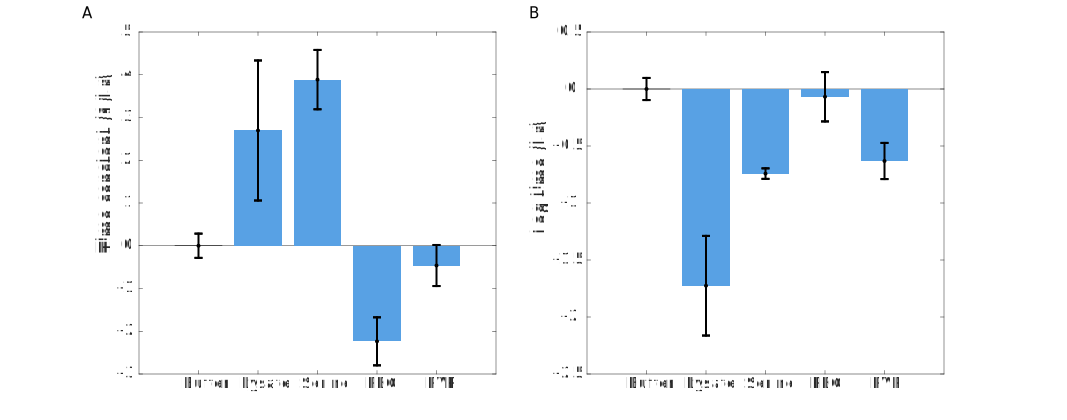
\includegraphics[width=0.8\textwidth]{figs/ch05/barCharts.pdf}
\label{fig:tht-all-conditions}
\end{figure}

% Recreating what I did to make these plots.  From Matlab script, loaded 
%j27 = load('C:\Users\bit\Desktop\sophie\time course fits\170127\170127_workspacefinal.mat');
%f19 = load('C:\Users\bit\Desktop\sophie\time course fits\170219\170219_workspace_final.mat');
%f21 = load('C:\Users\bit\Desktop\sophie\time course fits\170221\170221_workspace_final.mat');
%f28 = load('C:\Users\bit\Desktop\sophie\time course fits\170228\170228_workspace_final.mat');
%m07 = load('C:\Users\bit\Desktop\sophie\time course fits\170307\170307_workspace_final.mat');
%which desktop was this?  Probably old lab desktop


%use `dataforpaper.mat' in ch05 folder

We then combined replicates from all timecourses by condition and took the final average and standard error of the mean for both fit parameters.  The results are shown in Fig.~\ref{fig:fitParams}.  I ran a one-factor ANOVA to reject the null hypothesis that all means were the same, and then two-sample t-tests on each pair of conditions to find which differences were statistically significant.  For the time constant, all pairs of conditions were significantly different from each other with $p < 0.05$ \emph{except} buffer-PVP.   For the lag time, all pairs of conditions were significantly different from each other with $p < 0.05$ \emph{except} buffer-PEG and serine-PVP.

\begin{table}[b!]
  \caption[Aggregation rate p-values for all crowding agents.]{Aggregation rate $k$ p-values for all crowding agents, two-tailed t-test.}
    \label{table:p-k-values-all}
    \begin{tabular}{p{4cm}|p{3.5cm}p{3cm}p{2cm}p{2cm}}
        &10 mg/mL cell lysate &  19\% w/v serine & 13\% PEG & 13\% PVP\\
      \hline
	No crowder   & 0.031 & $1.2 \times 10^{-6}$ & $6.6\times 10^{-4}$ &0.41\\
	10 mg/mL cell lysate   & N/A & 0.44 & 0.0010 &  0.022\\
     	19\% w/v serine & N/A  & N/A & $4.4\times 10^{-9}$ & $2.2\times 10^{-6}$\\
      	13\% PEG    & N/A & N/A  & N/A & 0.019\\
	%13\% PVP & HeLa & a & b & 125 & N/A\\
    \end{tabular}
\end{table}

\begin{table}[b!]
  \caption[Lag time p-values for all crowding agents.]{Lag time $T_\ell$ p-values for all crowding agents, two-tailed t-test.}
    \label{table:p-tl-values-all}
    \begin{tabular}{p{4cm}|p{3.5cm}p{3cm}p{2cm}p{2cm}}
        &10 mg/mL cell lysate &  19\% w/v serine & 13\% PEG & 13\% PVP\\
      \hline
	No crowder   & $5.4 \times 10^{-6}$ & $1.4 \times 10^{-8}$ & 0.77 &0.0012\\
	10 mg/mL cell lysate   & N/A & 0.0051 & 0.00041 &  0.0060\\
     	19\% w/v serine & N/A  & N/A & 0.0052 & 0.53\\
      	13\% PEG    & N/A & N/A  & N/A & 0.039\\
	%13\% PVP & HeLa & a & b & 125 & N/A\\
    \end{tabular}
\end{table}

\begin{table}[b!]
  \caption[Aggregation rate p-values for PEG.]{Aggregation rate $k$ p-values for PEG (\% w/v) , two-tailed t-test.}
    \label{table:p-k-values-peg}
    \begin{tabular}{p{2cm}|p{3cm}p{3cm}p{3cm}p{3cm}}
        &20\% &  13\% & 5\% & 0\% \\ \hline
	25\% & 0.0063 & 0.6167 & 0.0007 &0.8344\\
	20\% & N/A &0.0131 & 0.7539 & 0.0815\\
     	13\% & N/A  & N/A & 0.1196 & 0.6508\\
      	5\% & N/A & N/A  & N/A & 0.0681\\
    \end{tabular}
\end{table}

\begin{table}[b!]
  \caption[Lag time p-values for PEG.]{Lag time $T_\ell$ p-values for PEG (\% w/v) , two-tailed t-test.}
    \label{table:p-tl-values-peg}
    \begin{tabular}{p{2cm}|p{3cm}p{3cm}p{3cm}p{3cm}}
        &20\% &  13\% & 5\% & 0\% \\ \hline
	25\% & 0.0071 & 0.0412 & 0.7726 &0.0221\\
	20\% & N/A &0.5377 &  0.0206 & 0.1012\\
     	13\% & N/A  & N/A & 0.1322 & 0.0927\\
      	5\% & N/A & N/A  & N/A &0.2833\\
    \end{tabular}
\end{table}

\begin{table}[b!]
  \caption[Aggregation rate p-values for PVP.]{Aggregation rate $k$ p-values for PVP (\% w/v) , two-tailed t-test.}
    \label{table:p-k-values-peg}
    \begin{tabular}{p{2cm}|p{3cm}p{3cm}p{3cm}p{3cm}}
        &20\% &  13\% & 5\% & 0\% \\ \hline
	25\% & 0.8521 & 0.1327 & 0.4104 &0.1880\\
	20\% & N/A &0.6607 & 0.6530 & 0.6815\\
     	13\% & N/A  & N/A & 0.5991 & 0.8283\\
      	5\% & N/A & N/A  & N/A & 0.6902\\
    \end{tabular}
\end{table}

\begin{table}[b!]
  \caption[Lag time p-values for PVP.]{Lag time $T_\ell$ p-values for PVP (\% w/v) , two-tailed t-test.}
    \label{table:p-tl-values-pvp}
    \begin{tabular}{p{2cm}|p{3cm}p{3cm}p{3cm}p{3cm}}
        &20\% &  13\% & 5\% & 0\% \\ \hline
	25\% & $4.7\times 10^{-5}$ & 0.0133 & 0.0012 &0.0628\\
	20\% & N/A &0.2586 &  $8.6\times 10^{-06}$ & 0.0272\\
     	13\% & N/A  & N/A & 0.0018 & 0.0709\\
      	5\% & N/A & N/A  & N/A &0.6774\\
    \end{tabular}
\end{table}

%\begin{table}[b!]
%  \caption[Lag time p-values for all crowding agents.]{Lag time $T_\ell$ p-values for all crowding agents, two-tailed t-test.}
%    \label{table:p-tl-values-all}
%    \begin{tabular}{p{2cm}|p{2cm}p{2cm}p{2cm}p{2cm}p{2cm}}
%        & 25 & 20 & 13 & 5 & 0 \\
%      \hline
%	25 & $5.4 \times 10^{-6}$ & $1.4 \times 10^{-8}$ & 0.77 &0.0012&\\
%	20 & N/A & 0.0051 & 0.00041 &  0.0060&\\
%     	13 & N/A  & N/A & 0.0052 & 0.53&\\
%      	5 & N/A & N/A  & N/A & 0.039&\\
%     	0 & N/A & N/A  & N/A & 0.039&\\
%    \end{tabular}
%\end{table}

\begin{figure}
\caption{test}
\centering
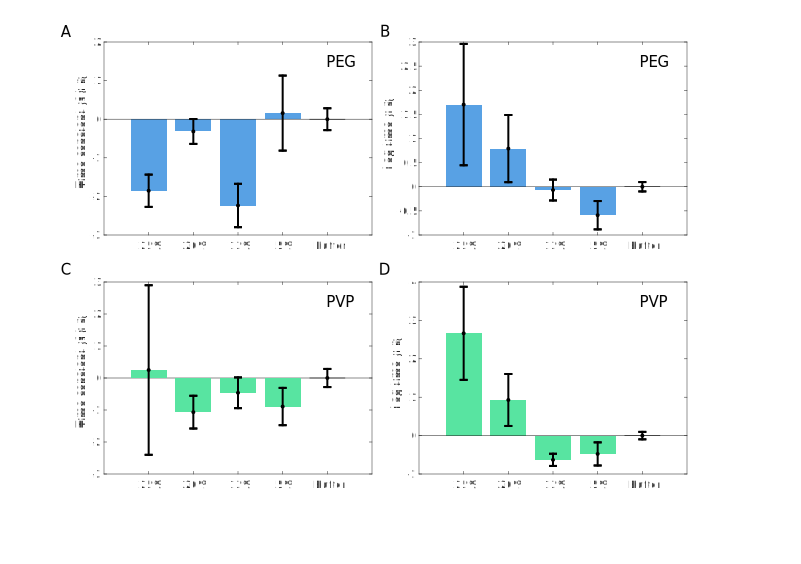
\includegraphics[width=\textwidth]{figs/ch05/peg-and-pvp-charts.pdf}
\label{fig:peg-pvp}
\end{figure}

I followed the same process for the timecourses involving the concentration series for PEG and PVP, but there were fewer significant differences between concentrations, as seen in Fig.~\ref{fig:peg-pvp}.  The ANOVA for the PEG time constants gave $p=0.0024$ with the t-test showing differences between: buffer-25\% PEG, buffer-13\% PEG, and 25\% PEG-20\% PEG. The ANOVA for the PEG lag times was likewise significant with $p = 0.0102$.  The significant pairs were: buffer-25\% PEG, buffer-20\% PEG, buffer-5\% PEG, and 25\% PEG-13\% PEG.

For PVP, there were no significant differences in the time constant.  For the lag time, after the ANOVA and t-tests, there were differences between: buffer and everything except 5\% PVP, 25\% PVP and everything but 20\% PVP, and 20\%PVP-13\% PVP.

For both conditions, it looks roughly like the lag time increases with the crowder concentration, but given the large error bars, I wouldn't read too much into it.  The time constants don't follow any particular trend and are mostly indistinguishable anyway.

We tested the effects of pH on FG124 aggregation by running several experiments in buffer at varying pH.  We ran six replicates of each condition, for pH values between 5 and 8.  No significant differences were found in the lifetimes or lag times of any pH condition.  Results are summarized in Table \ref{table:FG124-pH}. We concluded that aggregation is not affected by pH in the range 5-8.

\begin{table}[b!]
  \caption{FG124 aggregation lifetime and lag time with varying pH. Each condition run with 6 replicates in PTB buffer.  One-way ANOVAs show no statistically significant differences between conditions.  Standard errors are shown.}
    \label{table:FG124-pH}
    \begin{tabular}{p{1cm}p{3cm}p{3cm}}
      pH & Lifetime $\tau$ (hr) & Lag time $T_{lag}$ (hr) \\
      \hline
      5 & $0.34 \pm 0.09$ & $6.8 \pm 0.1$ \\
      6 & $0.35 \pm 0.12$ & $6.2 \pm 0.2$ \\
      7 & $0.38 \pm 0.14$ & $6.8 \pm 0.4$ \\
      8 & $0.50 \pm 0.14$ & $6.6 \pm 0.2$ \\
    \end{tabular}
\end{table}

\subsection{Discussion}

\section{NMR relaxation measurements}
\subsection{Methods}
\subsection{Results}
\subsection{Discussion}

\section{Fluorescence spectra}
We hypothesized that the crowder-dependent difference in aggregation might arise from the aromatic ring in PVP, which could interact with the phenylalanine in FG124 in a ring-stacking interaction.  To test this idea, I collected emission spectra of fresh and aggregated FG124 in PEG and PVP crowders near the phenylalanine peak wavelength (see Fig. \ref{fig:FG124-fresh-vs-agg}). 
\subsection{Methods}
FG124 was purified as described above and stored in PTB with 7M GuHCl.  Immediately before use, 130 uL of 520 uM FG124 was desalted with a Zeba spin desalting column to remove the GuHCl.  The resulting stock was used in the crowder samples, which had a final concentration of 340 uM Fg124.  I used the shared-instrumentation fluorimeter.  I tested PTB, 5\% PEG (MW, source, purity?) in PTB, and 5\% PVP (same questions?) in PTB as blanks.  I measured 340 uM FG124 in PTB and the two crowders as well.  Between runs, I cleaned the cuvette (micro quartz cuvette from Kaar lab (sample volume?)) with ethanol 3x, then 5x with DI water, and gently blotted the outside with ethanol.  Fluorimeter settings: 4 nm slits, 1000 V PMT, excitation wavelength of 240 nm.  Step size  = 1nm, average over 2 runs.  After taking this data with fresh FG124, I let the samples sit at room temp overnight to aggregate (no shaking) and most were cloudy in the morning.  I took similar data with the aggregated samples.  I needed to rinse with 7M GuHCl, let soak in 7M GuHCl for 5 minutes, and then perform the same cleaning procedure as the previous day in order to remove the aggregates from the cuvette.
\subsection{Results}
Only 5\% PEG and PVP in PTB were tested because PEG has a peak near the FG124 peak which dominates at higher PEG concentrations.  Data were normalized by averaging over two runs and subtracting a blank run (containing crowder and buffer but no protein).
\begin{figure}
\caption{Emission scan of fresh and aggregated FG124 in crowded conditions.  Data normalized by subtracting blank sample.}
\centering
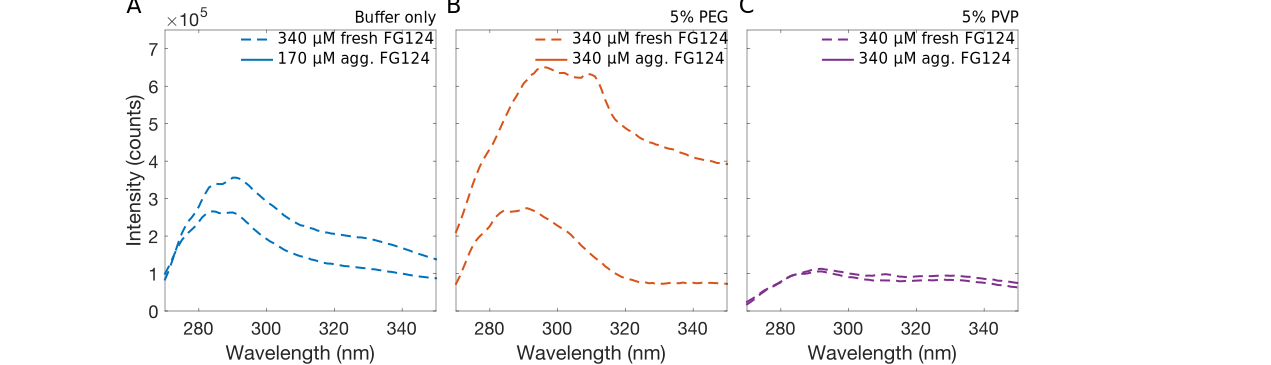
\includegraphics[width=1.1\textwidth]{figs/ch05/FG124-fresh-vs-agg}
\label{fig:FG124-fresh-vs-agg}
\end{figure}
The PEG sample showed the largest difference upon aggregation, both in peak height and location.  Figure \ref{fig:stacked-FG124-fluorimetry} shows the same data, normalized to a maximum amplitude of one and offset, in order to emphasize the changes in peak shape.
\begin{figure}
\caption{Emission scan of phenylalanine, FSFG, and FG124. Excited at 240 nm.  Phe data is not mine, need to check reference. Data normalized to a maximum amplitude of 1.}
\centering
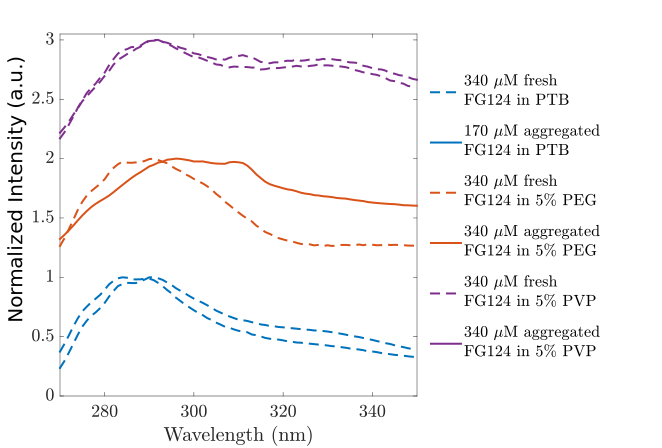
\includegraphics[width=\textwidth]{figs/ch05/stacked-FG124-fluorimetry}
\label{fig:stacked-FG124-fluorimetry}
\end{figure}
In both crowder conditions, but not in the buffer condition, a small peak appears in the aggregated FG124 near 310 nm.

Additionally, I compared the phenylalanine peaks in FSFG and fresh and aggregated FG124 to those of pure phenylalanine \cite{zotero-5177}, as seen in Fig. \ref{fig:phe-comparison}.  Data are blanked and normalized to a maximum intensity of one.  The peak slightly shifts toward longer wavelengths as the data progress from phenylalanine to FSFG to fresh and aggregated FG124.
\begin{figure}
\caption{Emission scan of phenylalanine, FSFG, and FG124. Excited at 240 nm.  Phe data is not mine, need to check reference. Data normalized to a maximum amplitude of 1.}
\centering
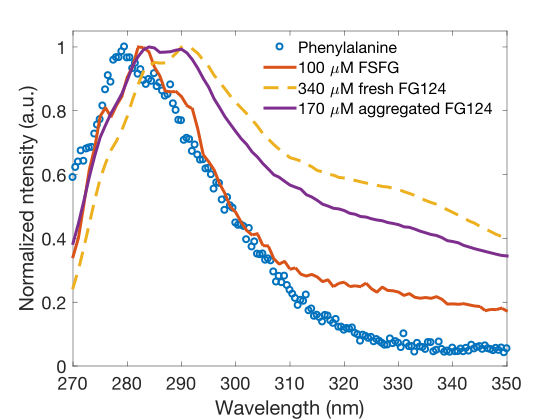
\includegraphics[width=0.5\textwidth]{figs/ch05/phe-comparison}
\label{fig:phe-comparison}
\end{figure}
I also measured PEG and PVP absorbance near 240 nm (see Fig.~\ref{fig:crowder-absorbance}).  PVP has a very high absorbance in that range, which might explain why the recorded counts were lowest for the PVP conditions.
\begin{figure}
\caption{Absorbance of 5\% PEG and PVP solutions in PTB.  Normalized by subtracting PTB absorbance.}
\centering
\includegraphics[width=0.5\textwidth]{figs/ch05/crowder-absorbance}
\label{fig:crowder-absorbance}
\end{figure}
\subsection{Discussion}

\section{Conclusions}

It's possible that the differences in aggregation time between PEG and PVP come from changes in viscosity.  The two samples do have widely different viscosity, as measured by Steve Whitten.  A 13\% PEG solution in PTB has a dynamic viscosity of 15.87 mPa s, while that of a 13\% PVP solution in PTB is 7.34 mPa s.  The literature doesn't entirely agree on what happens to aggregation as a function of viscosity, but what we see could be due to that change.  (Check in lab book where I have lit search notes.)
